\documentclass[10pt,xcdraw]{article}

\usepackage[es-tabla]{babel}
\usepackage{parskip}
\usepackage[capitalise, noabbrev]{cleveref}
\crefname{table}{\spanishtablename}{\spanishtablename}



\title{
	\textbf{
		Desarrollo de un modelo fundacional estocástico basado en procesos Gaussianos para la clasificación de bioseñales EEG en el diagnóstico asistido del TDAH.
	}
	}
\author{
	Julián David Pastrana Cortés, M.Sc.
	}


\date{} % Carga el preámbulo
\begin{document}
	%%%%%%%%%%%%%%%%%%%%%%%%%%%%%%%%%% PORTADA %%%%%%%%%%%%%%%%%%%%%%%%%%%%%%%%%%%%%%%%%%%%
\vspace*{0.5cm}
\begin{center}
	\newcommand{\HRule}{\rule{\linewidth}{0.5mm}}
	\vspace*{-1.5cm}
	% \textsc{\huge Universidad Tecnológica\\ \vspace{5px} de Pereira}\\[1.5cm]
	% 
\includegraphics[width=0.2\textwidth]{imagenes/Logo_UTP.png}
	% \vspace{1.5cm}
	\textsc{\LARGE Informe de actividades en el marco del programa: \\ 
		\vspace{0.4cm}
		ALIANZA CIENTÍFICA CON ENFOQUE COMUNITARIO PARA MITIGAR BRECHAS DE ATENCIÓN Y MANEJO DE TRASTORNOS MENTALES RELACIONADOS CON IMPULSIVIDAD EN COLOMBIA
		}\\
	\vspace{2cm}
	\HRule \\[0.4cm]
	{ \bfseries Nombre: Julián David Pastrana Cortés }\\[0.4cm]
	{ \bfseries Contrato de servicios: 5551 }\\[0.4cm]
	\vspace{1.5cm}
	
\includegraphics[width=0.28\textwidth]{imagenes/LogoU.png}
	
\includegraphics[width=0.35\textwidth]{imagenes/logo_automatica.png}
	\HRule \\[1.5cm]
	\vspace{1.5cm}
	\vspace*{0.5cm}
	\textsc{\textbf{\Large Grupo de investigación en Automática } }\\
	\vspace{3.5cm} 
	\begin{center}
		{\large \today}
	\end{center}
\end{center}
\newpage
   % Carga la portada y otros elementos de layout
	
	\tableofcontents 
	\newpage
	
	\section{Información general del contrato}
	\begin{table}[H]
		\centering
		\begin{tabular}{>{\arraybackslash}m{8cm} >{\arraybackslash}m{6.5cm}}
			\toprule
			\textbf{Rol} & \vspace{2mm}Contratista - Estudiante de Doctorado\vspace{2mm}\\\hline
			\vspace{2mm}
			\textbf{Contrato de servicios No.}\vspace{2mm} & \vspace{2mm} 5551 de 2025\vspace{2mm}\\\hline
			\vspace{2mm}
			\textbf{Objeto del contrato} \vspace{2mm} & \vspace{2mm} Prestación de servicios profesionales para el Desarrollo de metodología de gamificación para entrenamiento de niños con trastornos de impulsividad ALIANZA CIENTÍFICA CON ENFOQUE COMUNITARIO PARA MITIGAR BRECHAS DE ATENCIÓN Y MANEJO DE TRASTORNOS MENTALES RELACIONADOS CON IMPULSIVIDAD EN COLOMBIA - ACEMATE MINCIENCIAS CONTRATO 790-2023 
			\vspace{2mm}\\\hline
			\textbf{Período del informe} & \vspace{2mm} 01 de marzo de 2025 al 31 de marzo de 2025\vspace{2mm}\\\hline
		\end{tabular}
	\end{table}
	
	\subsection{Descripción general de la vinculación}
	Como resultado de la vinculación se contribuye al alcance de el objetivo 3 del programa de investigación: ALIANZA CIENTÍFICA CON ENFOQUE COMUNITARIO PARA MITIGAR BRECHAS DE ATENCIÓN Y MANEJO DE TRASTORNOS MENTALES RELACIONADOS CON IMPULSIVIDAD EN COLOMBIA
	
	\subsection{Objetivo general}
	Desarrollar una metodología de gamificación para entrenamiento de niños con trastornos de impulsividad ALIANZA CIENTÍFICA CON ENFOQUE COMUNITARIO PARA MITIGAR BRECHAS DE ATENCIÓN Y MANEJO DE TRASTORNOS MENTALES RELACIONADOS CON IMPULSIVIDAD EN COLOMBIA - ACEMATE MINCIENCIAS CONTRATO 790-2023.
	
	
	\section{Metodología}

Para dar cumplimiento a cada uno de los objetivos específicos, se propone la siguiente metodología, la cual estará dividida en tres fases (una por cada objetivo):

\subsection*{Fase 1: Diseño y Desarrollo del Modelo Fundacional para la Clasificación de Señales EEG}
\textbf{Objetivo específico 1:} Diseñar y desarrollar un modelo fundacional para la clasificación de señales biológicas relacionadas con registros EEG, que aproveche datos no etiquetados en la etapa de autoaprendizaje y datos etiquetados para su ajuste fino.

\begin{enumerate}
	\item \textbf{Actividad 1.1: Recopilación y Preprocesamiento de Datos EEG}\\
	Se recopilará un conjunto de registros EEG, provenientes de diversas fuentes, y se organizarán tanto bases de datos etiquetadas como no etiquetadas. Se realizará un preprocesamiento inicial que incluya la eliminación de artefactos, la normalización de los datos y la sincronización de las señales para asegurar la homogeneidad en la tasa de muestreo y el número de canales.
	
	\item \textbf{Actividad 1.2: Desarrollo del Modelo Fundacional}\\
	Se diseñará y desarrollará un modelo fundacional empleando técnicas de autoaprendizaje para extraer representaciones generales de las señales EEG. Posteriormente, se aplicará un ajuste fino utilizando los datos etiquetados para optimizar la capacidad del modelo en la clasificación de individuos con TDAH.
	
	\item \textbf{Actividad 1.3: Validación Interna del Modelo}\\
	Se validará el desempeño del modelo fundacional mediante métricas de clasificación. Se ajustarán los hiperparámetros en función de los resultados obtenidos, garantizando la adaptabilidad del modelo a nuevos escenarios clínicos.
\end{enumerate}

\subsection*{Fase 2: Implementación de la Herramienta de Predicción Estocástica Basada en Procesos Gaussianos}
\textbf{Objetivo específico 2:} Implementar una herramienta de predicción estocástica basada en procesos Gaussianos, que permita modelar la incertidumbre en la predicción del modelo fundacional.

\begin{enumerate}
	\item \textbf{Actividad 2.1: Investigación de Procesos Gaussianos para Modelar Incertidumbre}\\
	Realizar una revisión bibliográfica sobre técnicas basadas en procesos Gaussianos en el ámbito de datos biomédicos y EEG, identificando métodos adecuados para cuantificar la incertidumbre en las predicciones.
	
	\item \textbf{Actividad 2.2: Integración del Componente Gaussianos en el Modelo}\\
	Desarrollar e integrar en el modelo fundacional un módulo basado en procesos Gaussianos que estime la incertidumbre asociada a cada predicción, proporcionando una medida cuantitativa de la confiabilidad diagnóstica.
	
	\item \textbf{Actividad 2.3: Validación de la Herramienta Estocástica}\\
	Validar la herramienta de predicción estocástica mediante pruebas en un conjunto de datos independiente, evaluando la precisión del modelo y la utilidad de la estimación de incertidumbre para el diagnóstico asistido del TDAH.
\end{enumerate}

\subsection*{Fase 3: Elaboración de Estrategias para el Manejo de Características Faltantes}
\textbf{Objetivo específico 3:} Elaborar una estrategia para el manejo de características faltantes que complemente y extienda el modelo fundacional para tratar señales biológicas con información faltante.

\begin{enumerate}
	\item \textbf{Actividad 3.1: Revisión y Análisis de la Variabilidad en los Datos EEG}\\
	Realizar una revisión de la literatura para identificar los principales desafíos asociados a la variabilidad en los conjuntos de datos EEG, tales como valores ausentes, diferencias en la tasa de muestreo, variaciones en el número de canales y el fenómeno de dataset shift.
	
	\item \textbf{Actividad 3.2: Desarrollo de Estrategias de Imputación y Normalización Adaptativa}\\
	Investigar y seleccionar métodos de imputación y normalización que permitan corregir las inconsistencias en los datos sin descartar información valiosa. Se evaluarán diversas técnicas para determinar la mejor estrategia.
	
	\item \textbf{Actividad 3.3: Integración de la Gestión de Características Faltantes en el Modelo}\\
	Incorporar las estrategias desarrolladas en la fase anterior al flujo de trabajo del modelo fundacional, de manera que se optimice la capacidad del modelo para manejar señales biológicas incompletas.
	
	\item \textbf{Actividad 3.4: Validación y Documentación de la Estrategia}\\
	Validar la efectividad de la estrategia de manejo de características faltantes mediante pruebas comparativas con datos de EEG, y documentar el proceso que sirva de guía para la implementación y futuras mejoras.
\end{enumerate}

	\section{Conjunto de Datos}

\subsection{Toadstool: Un conjunto de datos para el entrenamiento de máquinas de inteligencia emocional que juegan a Super Mario Bros}

El conjunto de datos de libre acceso Toadstool es una colección de registros en video, sensores e información demográfica obtenidos de diez individuos mientras jugaban Super Mario Bros. La selección de los participantes se realizó buscando una amplia variedad en cuanto a experiencia previa con videojuegos, incluyendo desde personas que apenas habían jugado alguno en su vida hasta aquellas con una extensa trayectoria desde la infancia, con edades comprendidas entre los 26 y 48 años. También se buscó mantener un balance en el género, participando cinco hombres y cinco mujeres. Los autores en \cite{toadstool} señalan la presencia de anomalías, tales como ninguna o muy poca actividad detectada por los sensores, así como diferencias significativas entre la actividad registrada al inicio y al final de las sesiones de juego.

El desempeño de los participantes fue evaluado según el número de niveles completados en un tiempo determinado y el número de muertes ocurridas durante la partida. Dicho puntaje se mantuvo en secreto entre los participantes para evitar que se rindieran o relajaran durante el juego. Adicionalmente, se les incentivó mediante una recompensa con el fin de mantener un desempeño competitivo. Un resumen de las características de los participantes se presenta en la \cref{tab:datos_participantes}.


\begin{table}[h!]
	\centering
	\resizebox{\textwidth}{!}{%
		\begin{tabular}{|c|c|c|c|c|c|c|c|}
			\hline
			\textbf{ID} & \textbf{Edad} & \textbf{Sexo} & \textbf{Mano dominante} & \shortstack{\textbf{Horas}\\\textbf{por semana}} & \shortstack{\textbf{Años}\\\textbf{de actividad}} & \shortstack{\textbf{Experiencia}\\\textbf{previa}} & \shortstack{\textbf{Puntaje}\\\textbf{del juego}} \\
			\hline
			0 & 26 & Hombre & Derecha  & 4--8 & 22 & Mucha  & 17,100 \\
			1 & 48 & Hombre & Izquierda & 0--1 & 1  & Poca   & 3,000  \\
			2 & 28 & Hombre & Derecha  & 0--1 & 0  & Ninguna& 300    \\
			3 & 32 & Hombre & Derecha  & 4--8 & 4  & Algo   & 13,300 \\
			4 & 32 & Mujer  & Derecha  & 0--1 & 5  & Algo   & 6,400  \\
			5 & 30 & Mujer  & Derecha  & 0--1 & 5  & Poca   & 2,700  \\
			6 & 35 & Hombre & Izquierda & 1--4 & 30 & Mucha  & 14,300 \\
			7 & 34 & Mujer  & Derecha  & 1--4 & 14 & Algo   & 3,800  \\
			8 & 31 & Mujer  & Derecha  & 0--1 & 2  & Poca   & 200    \\
			9 & 27 & Mujer  & Derecha  & 0--1 & 5  & Poca   & 10,600 \\
			\hline
		\end{tabular}%
	}
	\caption{Características demográficas y experiencia de los participantes en relación con su desempeño en el juego. Se incluyen datos como edad, sexo, lateralidad, dedicación semanal, años de experiencia, nivel de experiencia previa y puntaje obtenido.}
	\label{tab:datos_participantes}
\end{table}

En el conjunto de datos, se incluye para cada participante un video de su rostro durante la sesión de juego, grabado a una resolución de 640×480 píxeles y a 30 fotogramas por segundo. Además, se registran las acciones realizadas mediante el mando de juego para controlar al personaje, así como los datos recopilados por la pulsera Empatica E4. La Empatica E4 es un dispositivo que permite la adquisición en tiempo real de datos fisiológicos, como la actividad electrodérmica (EDA), el pulso de volumen sanguíneo (BVP), la temperatura de la piel y la aceleración en tres ejes \cite{garbarino2014empatica}.




	
	\section{Resultados}
	Versión final del estado del arte sobre modelos de detección del TDAH basados en modelos funcacionales y procesos Gaussianos redactado en una propuesta de doctorado. El documento se encuentra en la sección de anexos.
	
	Avance en el desarrollo de un modelo de inferencia basado en Procesos Gaussianos encadenados para la amplicación de la metodología de gamificación. Consiste en un conjunto de códigos en lenguaje Python.
	
	\section{Anexos}
% Include first page with a title overlay
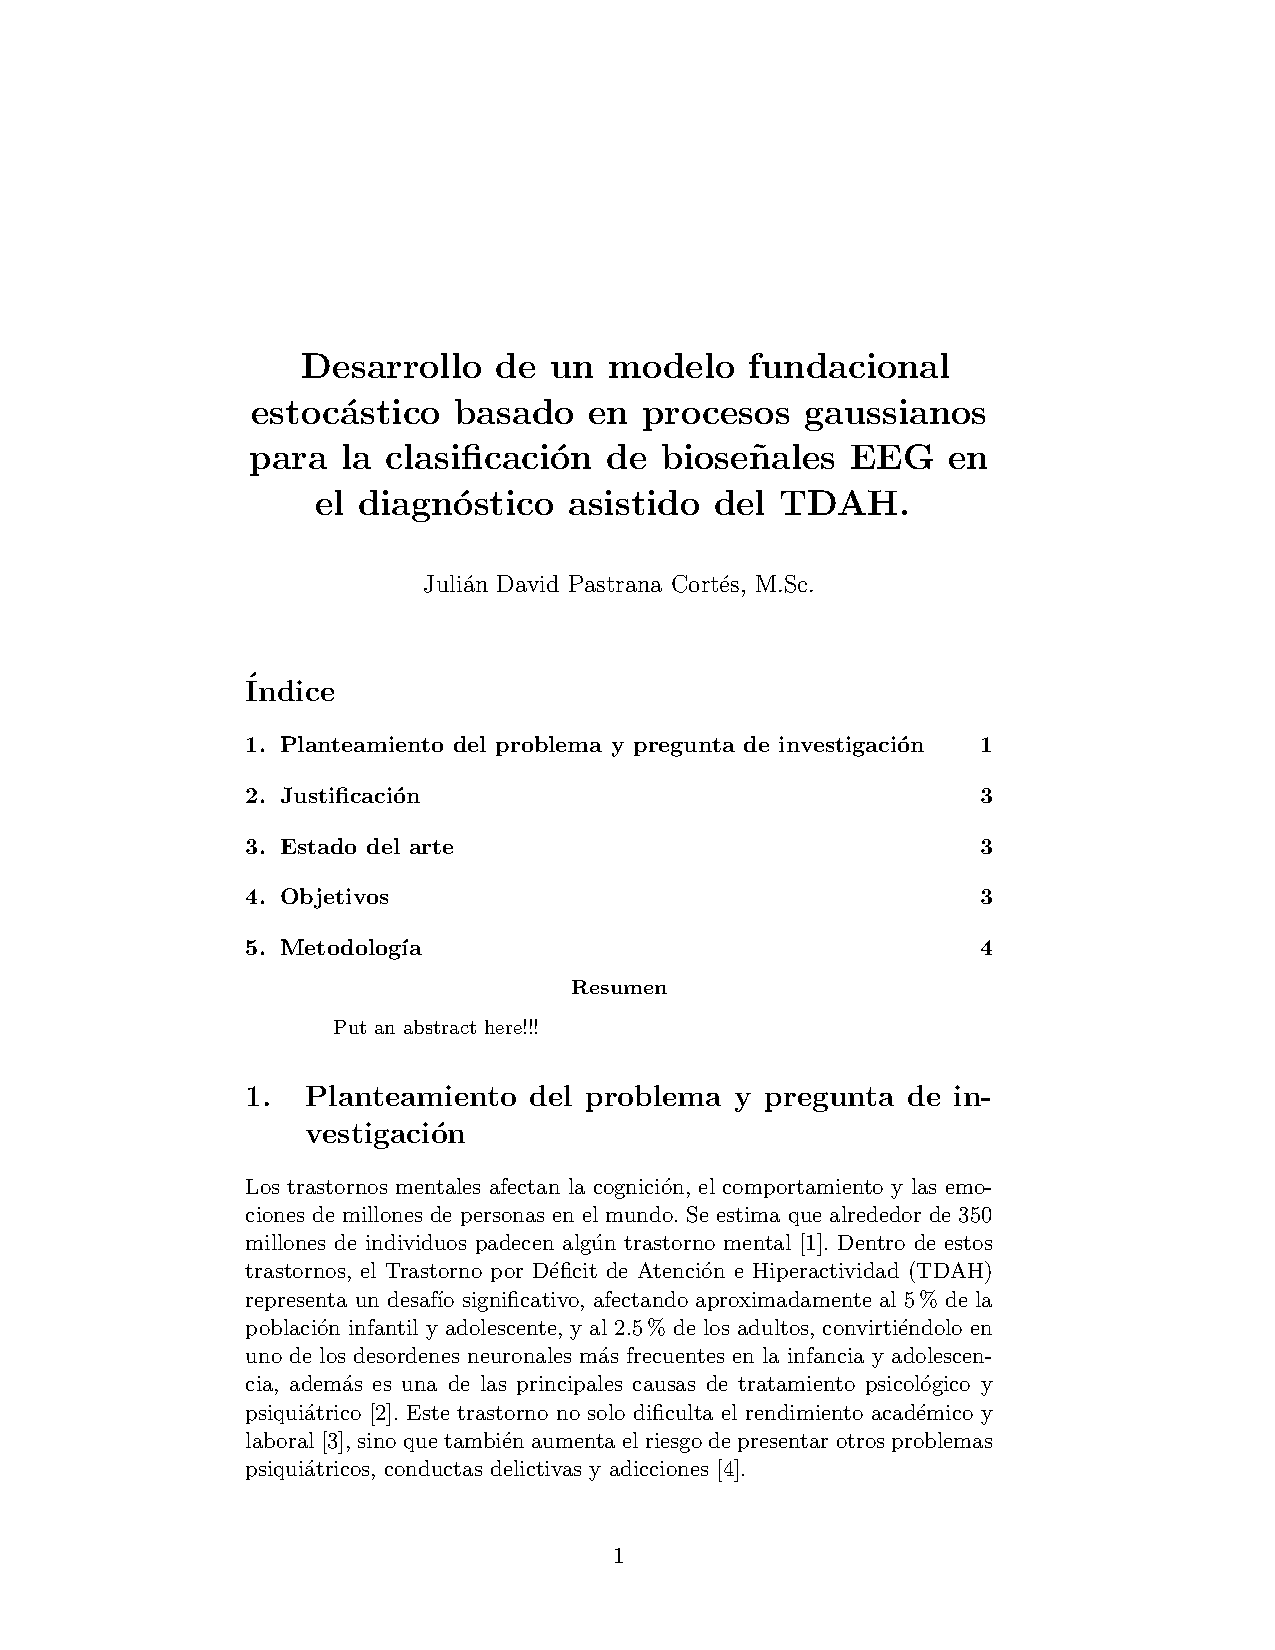
\includepdf[pages=1,
pagecommand={%
	\thispagestyle{plain}
		\Large\bfseries Propuesta doctorado
}
]{../propuesta_doctorado/main.pdf}
% Include remaining pages without any overlay
\includepdf[pages=2-last, pagecommand={}]{../propuesta_doctorado/main.pdf}

	\bibliographystyle{apalike}
	\bibliography{refs}
	
\end{document}
